\documentclass{standalone}

\usepackage{graphicx}
\usepackage{wrapfig}
\usepackage{lscape}
\usepackage{rotating}
\usepackage{epstopdf}

\begin{document}

We have been preparing a new robot platform, Aero (Figure
\ref{fig:aero}), for use in task 2 of the challenge. From our past
experience (DRC Finals 2015), we encountered problems
with shipments. Transportation of large and heavy robots are
cumbersome, requires early shipment and difficult due to customs and
board control regulations of countries. 



% During DRC finals 2015, 
% From our past
% experience in DRC, transportation of large robots that require to be shipped
% separately proved to be very difficult due to customs regulations of
% countries. 

%% It is comparatively much easier to transport a robot that
%% can be carried onto an airplane with us as carry-on luggages. 
It is comparatively much easier to transport a robot that
can be separated into modules and taken onto an airplane with project personnel.
% with us as carry-on luggages. 
Aero is designed to be light weight and modular. Compared to 
our HPR2 robot we showed in our first progress report, which weighs
approximately 90 kg, aero only weighs approximately 65 kg. It is 
made up of a mobile base, a lifter, and an arm module, which can each 
be separated and fit into suitcases for transportation. 

%Aero contains 2 degrees of freedom in the lifter and 6 degrees of freedom in the arm. 

The lifter in the Aero has 2 degrees of freedom while the arm has 6 degrees
of freedom. For carrying out task 2, we have fitted Aero's arm
with the same magnetic gripper used for HRP2. 




We have been considering and testing several designs of the mobile base, including the following configurations:
\begin{itemize}
	\item 4 active Mecanum wheels 
	\item 4 active tire wheels
	\item 2 	active tire wheels + 1 passive caster wheel
	\item 2 	active tire wheels + 2 passive omni wheels
\end{itemize}

Each configuration trades off maneuverability, ease of path planing,
and compatibility with different terrains. Currently we are making our
next version of the mobile base, and we will select the best
configuration for our final design based on the competition arena
ground surface type. 


\begin{figure}[h]
   \newcommand \ilenght{0.1}
   \newcommand \iheight{2.0in}
   \newcommand \iwidth{0.46\textwidth}
   \centering
{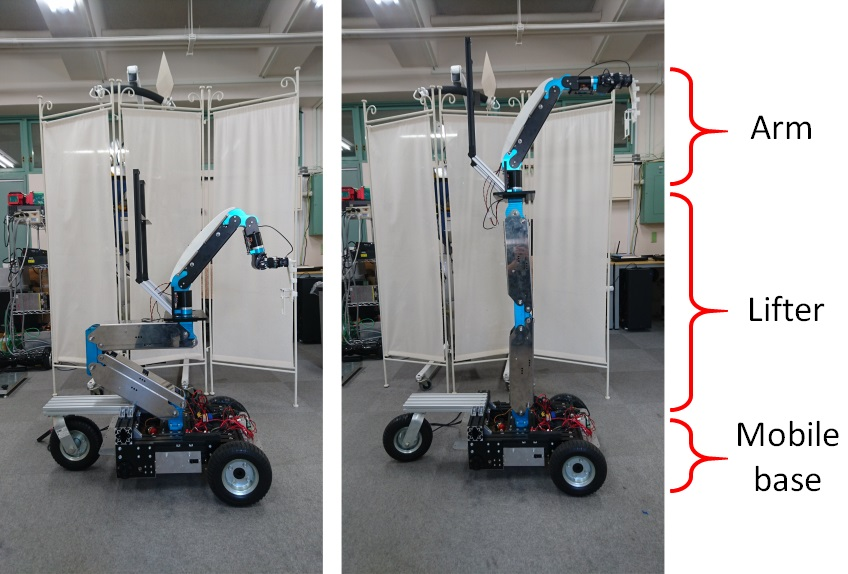
\includegraphics[width=\iwidth, height=\iheight]{sections/task2/images/aero.jpg}}\hspace{1.1em}%
   \caption{Our new robot platform, Aero. Left: lowered position. Right: extended position.}
   \label{fig:aero}
 \end{figure}

\end{document}
